\documentclass[tikz,border=8pt,multi=tikzpicture]{standalone}

\usepackage{amsmath}
\usepackage{bm}
\usepackage[T1]{fontenc}
\usepackage[scaled=0.95]{helvet}
\usetikzlibrary{arrows.meta,backgrounds,calc,fit,positioning}

% Keep mathematical symbols in Computer Modern while matching the website's
% palette and Helvetica-style prose labels.
\definecolor{diagramText}{HTML}{121212}
\definecolor{diagramMuted}{HTML}{4A4F55}
\definecolor{diagramBorder}{HTML}{CFD4D8}
\definecolor{diagramSurface}{HTML}{F4F5F7}
\definecolor{diagramPrimary}{HTML}{2B6CAF}
\definecolor{actionColor}{HTML}{7AA6FF}
\definecolor{stateColor}{HTML}{A568CD}
\definecolor{agentColor}{HTML}{F07A26}

\newcommand{\diagramlabel}[1]{{\sffamily\small\color{diagramText}#1}}
\newcommand{\tokenmath}[1]{{\normalsize$\bm{#1}$}}

\begin{document}

% Page 1: the ordinary causal sequence.
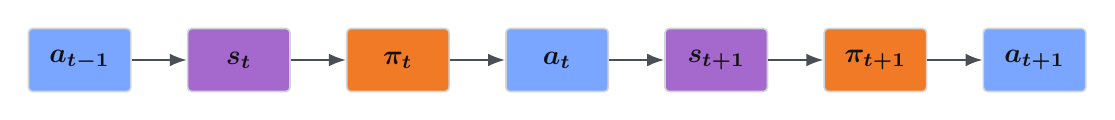
\begin{tikzpicture}[
  >=Latex,
  token/.style={
    draw=diagramBorder,
    text=diagramText,
    rounded corners=1.5pt,
    minimum width=13mm,
    minimum height=8mm,
    inner sep=2pt,
    line width=0.6pt,
    font=\small
  },
  action/.style={token, fill=actionColor},
  state/.style={token, fill=stateColor},
  agent/.style={token, fill=agentColor},
  flow/.style={->, draw=diagramMuted, line width=0.7pt}
]
\node[action] (linear-am1) {\tokenmath{a_{t-1}}};
\node[state, right=7mm of linear-am1] (linear-st) {\tokenmath{s_t}};
\node[agent, right=7mm of linear-st] (linear-pit) {\tokenmath{\pi_t}};
\node[action, right=7mm of linear-pit] (linear-at) {\tokenmath{a_t}};
\node[state, right=7mm of linear-at] (linear-st1) {\tokenmath{s_{t+1}}};
\node[agent, right=7mm of linear-st1] (linear-pit1) {\tokenmath{\pi_{t+1}}};
\node[action, right=7mm of linear-pit1] (linear-at1) {\tokenmath{a_{t+1}}};

\draw[flow] (linear-am1) -- (linear-st);
\draw[flow] (linear-st) -- (linear-pit);
\draw[flow] (linear-pit) -- (linear-at);
\draw[flow] (linear-at) -- (linear-st1);
\draw[flow] (linear-st1) -- (linear-pit1);
\draw[flow] (linear-pit1) -- (linear-at1);

\end{tikzpicture}

% Page 2: the same sequence folded into model-timestep columns.
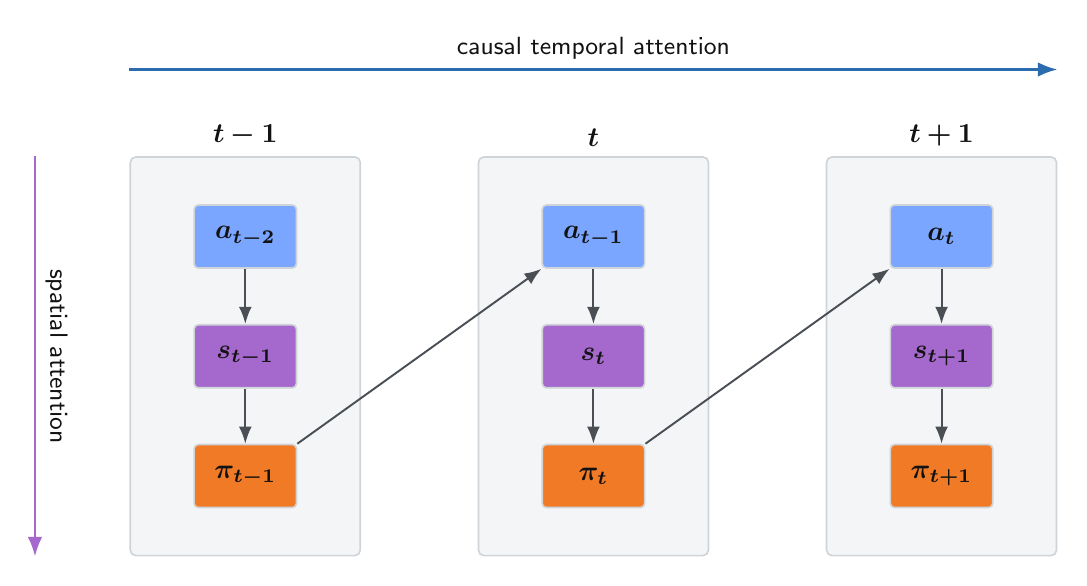
\begin{tikzpicture}[
  >=Latex,
  token/.style={
    draw=diagramBorder,
    text=diagramText,
    rounded corners=1.5pt,
    minimum width=13mm,
    minimum height=8mm,
    inner sep=2pt,
    line width=0.6pt,
    font=\small
  },
  action/.style={token, fill=actionColor},
  state/.style={token, fill=stateColor},
  agent/.style={token, fill=agentColor},
  timestep/.style={
    draw=diagramBorder,
    fill=diagramSurface,
    rounded corners=2pt,
    inner xsep=8mm,
    inner ysep=6mm,
    line width=0.6pt
  },
  flow/.style={->, draw=diagramMuted, line width=0.7pt},
  temporal axis/.style={->, draw=diagramPrimary, line width=0.9pt},
  spatial axis/.style={->, draw=stateColor, line width=0.9pt}
]
\node[action] (am2) {\tokenmath{a_{t-2}}};
\node[state, below=7mm of am2] (sm1) {\tokenmath{s_{t-1}}};
\node[agent, below=7mm of sm1] (pim1) {\tokenmath{\pi_{t-1}}};

\node[action, right=31mm of am2] (am1) {\tokenmath{a_{t-1}}};
\node[state, below=7mm of am1] (st) {\tokenmath{s_t}};
\node[agent, below=7mm of st] (pit) {\tokenmath{\pi_t}};

\node[action, right=31mm of am1] (at) {\tokenmath{a_t}};
\node[state, below=7mm of at] (st1) {\tokenmath{s_{t+1}}};
\node[agent, below=7mm of st1] (pit1) {\tokenmath{\pi_{t+1}}};

% Spatial information flow inside each model timestep.
\draw[flow] (am2) -- (sm1);
\draw[flow] (sm1) -- (pim1);
\draw[flow] (am1) -- (st);
\draw[flow] (st) -- (pit);
\draw[flow] (at) -- (st1);
\draw[flow] (st1) -- (pit1);

% The policy output becomes the action entering the following timestep.
\draw[flow] (pim1.north east) -- (am1.south west);
\draw[flow] (pit.north east) -- (at.south west);

% Timestep boxes are drawn behind their contents.
\begin{scope}[on background layer]
  \node[timestep, fit=(am2)(sm1)(pim1),
        label={[text=diagramText]above:{\tokenmath{t-1}}}] (box-m1) {};
  \node[timestep, fit=(am1)(st)(pit),
        label={[text=diagramText]above:{\tokenmath{t}}}] (box-t) {};
  \node[timestep, fit=(at)(st1)(pit1),
        label={[text=diagramText]above:{\tokenmath{t+1}}}] (box-p1) {};
\end{scope}

% Attention axes.
\draw[temporal axis]
  ($(box-m1.north west)+(0,11mm)$)
  -- node[above] {\diagramlabel{causal temporal attention}}
  ($(box-p1.north east)+(0,11mm)$);

\draw[spatial axis]
  ($(box-m1.north west)+(-12mm,0)$)
  -- node[midway, above, rotate=-90] {\diagramlabel{spatial attention}}
  ($(box-m1.south west)+(-12mm,0)$);

\end{tikzpicture}

\end{document}
